\chapter{傅立叶变换}
\section{从傅立叶级数到傅立叶变换}
我们将非周期函数看作是周期函数的一种特殊情况:周期趋向无穷。
\subsection{对于周期为1的函数}
\begin{align*}
	c_k=\hat{f}(k)=\int_0^1\ e^{-2\cdot \pi\cdot i\cdot k\cdot t}\cdot f(t)\ dt \\
	f(t)=\sum\limits_{k=-\infty}^{\infty}\ \hat{f}(k)\cdot e^{2\cdot \pi\cdot i\cdot k\cdot t}
\end{align*}
\begin{figure}[H]
	\centering
	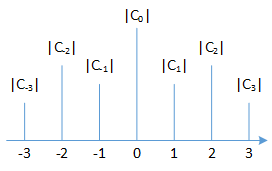
\includegraphics[width=0.4\textwidth]{assets/ft1.png}
	\caption{周期为$1$的函数是频谱图。由于$c_k$为复数形式,因此我们无法在图上画出,因此只能画出$c_k$的模。另外我们在第二节课的时候也学过,$c_k$是$y$轴对称的。}
\end{figure}
\begin{enumerate}
	\item 傅立叶变换是对傅立叶系数的一般化;
	\item Inverse 傅立叶变换是对傅立叶级数的一般化。
\end{enumerate}
\subsection{对于周期为T的函数}
$$
	c_k=\frac{1}{T}\cdot \int_{-\frac{T}{2}}^{\frac{T}{2}}\ e^{-2\cdot \pi\cdot i\cdot \frac{k}{T}\cdot t}\cdot f(t)\ dt
$$
$$
	f(t)=\sum\limits_{k=-\infty}^{\infty}\ \hat{f}(k)\cdot e^{2\cdot \pi\cdot i\cdot\cdot  \frac{k}{T}\cdot t}
$$

\begin{figure}[H]
	\centering
	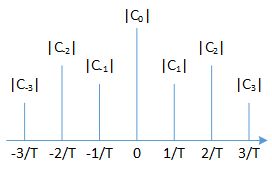
\includegraphics[width=0.4\textwidth]{assets/ft2.png}
	\caption{周期为$T$的函数的频谱图。由于周期为$T$,因此频率为$\frac{1}{T}$。当$T\rightarrow\infty$时,$\frac{1}{T}\rightarrow 0$,此时频谱会变得连续了。}
\end{figure}
\begin{enumerate}
	\item 这里为什么有个$\frac{1}{T}$???老师说从头开始推,他就不推了,你可以推推。
	\item 对于周期函数来说,积分的周期从哪里开始到哪里结束没人在意。
\end{enumerate}
\subsection{对于周期为$\infty$的函数}
只让$T\rightarrow \infty$不能得到傅立叶变换:
\begin{figure}[H]
	\centering
	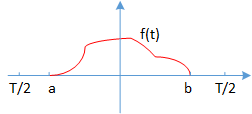
\includegraphics[width=0.4\textwidth]{assets/ft3.png}
	\caption{周期为$\infty$的函数的频谱图}
\end{figure}
\begin{align*}
	     & \hat{f}(k)                                                                                                       \\
	=    & \frac{1}{T}\cdot \int_{-\frac{T}{2}}^{\frac{T}{2}}\ e^{-2\cdot \pi\cdot i\cdot \frac{k}{T}\cdot t}\cdot f(t)\ dt \\
	=    & \frac{1}{T}\cdot \int_{a}^{b}\ e^{-2\cdot \pi\cdot i\cdot \frac{k}{T}\cdot t}\cdot f(t)\ dt                      \\
	\leq & \frac{1}{T}\cdot \int_{a}^{b}\ |e^{-2\cdot \pi\cdot i\cdot \frac{k}{T}\cdot t}|\cdot |f(t)|\ dt                  \\
	=    & \frac{1}{T}\cdot \int_{a}^{b}\ Mod\{[\cos^2(-2\cdot \pi\cdot i\cdot \frac{k}{T}\cdot t)                          \\
	+    & \sin^2(-2\cdot \pi\cdot i\cdot \frac{k}{T}\cdot t)]^{\frac{1}{2}}\}\cdot |f(t)|\ dt                              \\
	=    & \frac{1}{T}\cdot \int_a^b 1\cdot |f(t)|\ dt                                                                      \\
	=    & \frac{M}{T}
\end{align*}
即对所有$c_k=\hat{f}(k)$都有:$c_k\leq \frac{M}{T}$。

$M$是该函数绝对值的积分,是有限值。如果$T\rightarrow \infty$,那么$c_k\rightarrow 0$;则所有傅立叶系数全都没有意义。
\section{新符号$\mathcal{F}$}
由于$c_k\leq \frac{M}{T}$,$c_k$和$T$成反比,所以我们想到把$T$和$c_k$相乘,这样就不会出现上面的问题了。

在傅立叶级数中,$\mathcal{F}f(k)=c_k$,现在令$\mathcal{F}f(\frac{k}{T})=c_k\cdot T$,这是傅立叶变换线性的一种体现。

\begin{align*}
	     & \mathcal{F}f(\frac{k}{T})   =    c_k\cdot T                                                                                      \\
	=    & \int_{-\frac{T}{2}}^{\frac{T}{2}}\ e^{-2\cdot \pi\cdot i\cdot \frac{k}{T}\cdot t}\cdot f(t)\ dt                                  \\
	f(t) & =\sum\limits_{k=-\infty}^{\infty}\ \mathcal{F}f(\frac{k}{T})\cdot e^{2\cdot \pi\cdot i\cdot \frac{k}{T}\cdot t}\cdot \frac{1}{T}
\end{align*}

取值间隔为$\frac{1}{T}\rightarrow 0$,趋于连续变量,现在用连续变量$s$来表示$\frac{k}{T}$:
\begin{align*}
	  & \mathcal{F}f(s)                                                                       \\
	= & c_k\cdot T                                                                            \\
	= & \int_{-\frac{T}{2}}^{\frac{T}{2}}\ e^{-2\cdot \pi\cdot i\cdot s\cdot t}\cdot f(t)\ dt \\
	= & \int_{-\infty}^{\infty}\ e^{-2\cdot \pi\cdot i\cdot s\cdot t}\cdot f(t)\ dt
\end{align*}
由于$\frac{k}{T}$被替换为连续变量$s$,因此傅立叶级数中的多项式之和被替换成积分,其中$\frac{1}{T}$为$\Delta s$,即$ds$:
\begin{align*}
	f(t)   =  \int_{-\infty}^{\infty}\ \mathcal{F}f(s)\cdot e^{2\cdot \pi\cdot i\cdot s\cdot t}\ ds
\end{align*}
\section{傅立叶变换和Inverse 傅立叶变换}
\subsection{傅立叶变换}
\subsubsection{两种书写方式}
\begin{enumerate}
	\item $\mathcal{F}f(s)=\int_{-\infty}^{\infty}\ e^{-2\cdot \pi\cdot i\cdot s\cdot t}\cdot f(t)\ dt$;
	\item $F(s)=\int_{-\infty}^{\infty}\ e^{-2\cdot \pi\cdot i\cdot s\cdot t}\cdot f(t)\ dt$。
\end{enumerate}
\subsubsection{注解}
傅立叶变换在频域上分析信号,因此自变量为频率变量$s$。
\subsection{Inverse 傅立叶变换}
\subsubsection{两种书写方式}
\begin{enumerate}
	\item $\mathcal{F}^{-1}g(s)=\int_{-\infty}^{\infty}\ g(s)\cdot e^{2\cdot \pi\cdot i\cdot s\cdot t}\ ds$;
	\item $f(t)=\int_{-\infty}^{\infty}\ \mathcal{F}f(s)\cdot e^{2\cdot \pi\cdot i\cdot s\cdot t}\ ds$。
\end{enumerate}
\subsubsection{注解}
Inverse 傅立叶变换在时域上分析信号,因此自变量为时间变量$t$。
\subsection{傅立叶变换和Inverse 傅立叶变换之间的关系}
\begin{enumerate}
	\item $\mathcal{F}^{-1}\mathcal{F}f=f$
	\item $\mathcal{F}\mathcal{F}^{-1}g=g$
\end{enumerate}
\subsection{零点的值}
\begin{align*}
	  & \mathcal{F}f(0)                                                             \\
	= & \int_{-\infty}^{\infty}\ e^{-2\cdot \pi\cdot i\cdot 0\cdot t}\cdot f(t)\ dt \\
	= & \int_{-\infty}^{\infty}\ f(t)\ dt                                           \\
	  & \mathcal{F}^{-1}g(0)                                                        \\
	= & \int_{-\infty}^{\infty}\ e^{-2\cdot \pi\cdot i\cdot s\cdot 0}\cdot g(s)\ ds \\
	= & \int_{-\infty}^{\infty}\ g(s)\ ds
\end{align*}
\section{傅立叶变换实例}
\subsection{$\Pi$函数}
$$
	\pi(t)=
	\begin{cases}
		1 & |t|\leq\frac{1}{2} \\
		0 & |t|\geq\frac{1}{2}
	\end{cases}
$$
\begin{figure}[H]
	\centering
	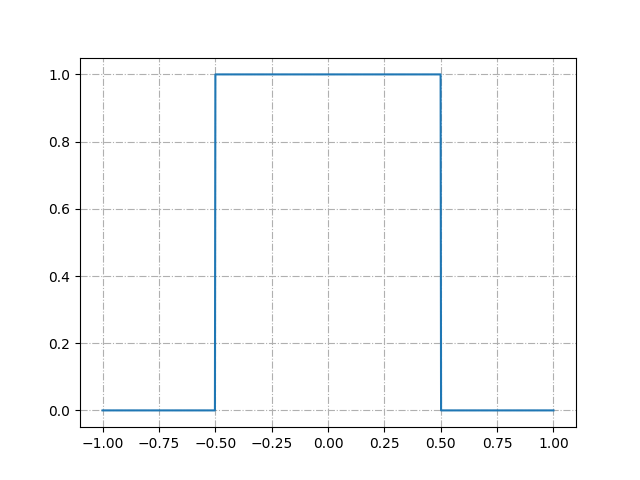
\includegraphics[width=0.4\textwidth]{assets/Figure_3.png}
	\caption{$\Pi$函数}
\end{figure}
\begin{align*}
	  & \mathcal{F}\ \Pi(s)                                                                                                            \\
	= & \int_{-\infty}^{\infty}\ e^{-2\cdot \pi\cdot i\cdot s\cdot t}\cdot \Pi(t)\ dt                                                  \\
	= & \rsx{-\frac{1}{2\cdot\pi\cdot i\cdot s}\cdot e^{-2\cdot \pi\cdot i\cdot s\cdot t}}_{-\frac{1}{2}}^{\frac{1}{2}}                \\
	= & -\frac{1}{2\cdot\pi\cdot i\cdot s}\cdot e^{- \pi\cdot i\cdot s}+\frac{1}{2\cdot\pi\cdot i\cdot s}\cdot e^{- \pi\cdot i\cdot s} \\
	= & \frac{1}{\pi\cdot s}\cdot \frac{e^{\pi\cdot i\cdot s}-e^{- \pi\cdot i\cdot s}}{2\cdot i}                                       \\
	= & \frac{\sin(\pi\cdot s)}{\pi\cdot s}                                                                                            \\
	= & \sinc(\pi\cdot s)
\end{align*}
\begin{figure}[H]
	\centering
	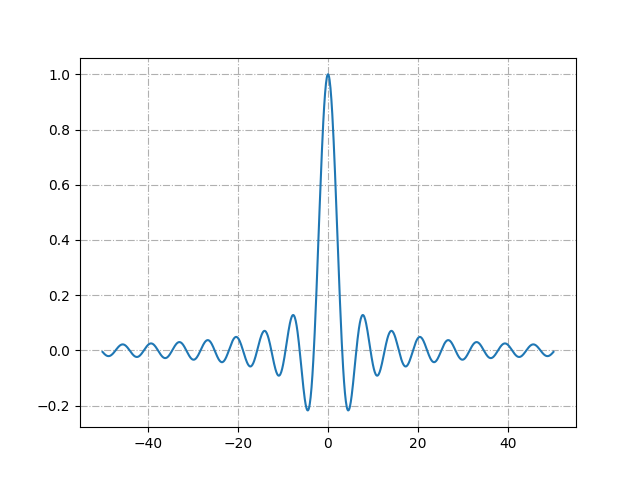
\includegraphics[width=0.4\textwidth]{assets/Figure_2.png}
	\caption{$\sinc$函数}
\end{figure}
\subsection{$\Lambda$函数}
\begin{figure}[H]
	\centering
	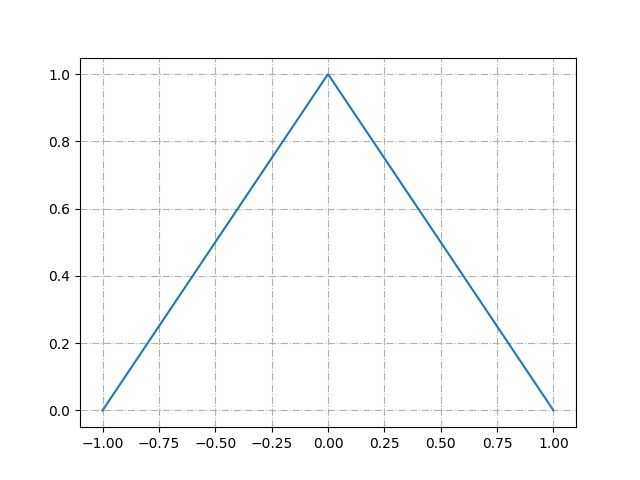
\includegraphics[width=0.4\textwidth]{assets/Figure_4.png}
	\caption{$\Lambda$函数}
\end{figure}
\begin{align*}
	  & \mathcal{F}\ \Lambda(s)                                                                                                              \\
	= & \int_{-\infty}^{\infty}\ e^{-2\cdot \pi\cdot i\cdot s\cdot t}\cdot \Lambda(t)\ dt                                                    \\
	= & \int_{-1}^{0}\ e^{-2\cdot \pi\cdot i\cdot s\cdot t}\cdot (1+t)\ dt+\int_{0}^{1}\ e^{-2\cdot \pi\cdot i\cdot s\cdot t}\cdot (1-t)\ dt \\
	= & \frac{\cos^2(\pi\cdot s)}{\pi\cdot s}                                                                                                \\
	= & \sinc^2(\pi\cdot s)
\end{align*}
\subsection{$\Lambda$与$\Pi$之间的关系}
Every 信号 has a spectrum, the spectrum determines the 信号.

我们可以看到$\Pi$函数和$\Lambda$函数经过傅立叶变换后奇妙的平方关系。事实上,通过后面利用傅立叶变换证明大数定律可知,任何信号经过几次傅立叶变换之后的频谱图都会变得越来越像一个“钟形”,即正态分布的样子。往后看一看卷积相关的知识可以看到:
$$
	\mathcal{F}f(\pi*\pi)=(\mathcal{F}f\ \pi)\cdot(\mathcal{F}f\ \pi)=\sinc^2=\mathcal{F}\ \Lambda
$$

一般情况下,$f*g$都比单独的$f$或$g$要平滑一些。就好像矩形函数$\Pi$没有三角函数$\Lambda$平滑一些。
\section{傅立叶变换的对称性}
\subsection{时域和频域之间的对称关系}
\begin{enumerate}
	\item 傅立叶变换从时域转换到频域;
	\item Inverse 傅立叶变换从频域转换到时域。
\end{enumerate}
\subsection{反转信号}
令$f^-(t)=f(-t)$,$f^-(t)$即为$f(t)$的反转。

\subsection{对偶定理}
\subsubsection{对偶定理1}
由反转函数的定义得:
$$
	\mathcal{F}f(-s)=(\mathcal{F}f)^-(s)
$$

又因为:
\begin{align*}
	  & \mathcal{F}f(-s)                                                           \\
	= & \int_{-\infty}^{\infty}\ e^{2\cdot \pi\cdot i\cdot s\cdot t}\cdot f(t)\ dt \\
	= & \mathcal{F}^{-1}f(s)
\end{align*}

所以:
\begin{equation}\label{du1}
	(\mathcal{F}f)^-=\mathcal{F}^{-1}f
\end{equation}

函数傅立叶变换的反转等于对该函数进行Inverse 傅立叶变换。

在积分中,变量叫什么不重要。在\ref{du1}中,积$s$和积$t$是一样的效果。

傅立叶变换的变量是频域变量$s$。

$\mathcal{F}^{-1}f$中对时域进行了Inverse 傅立叶变换。And this makes no sense. But, math is math, nobody cares.

\subsubsection{对偶定理2}
\begin{align*}
	  & \mathcal{F}(f^-(t))                                                                            \\
	= & \int_{-\infty}^{\infty}\ e^{-2\cdot \pi\cdot i\cdot s\cdot t}\cdot f(-t)\ dt                   \\
	= & \int_{\infty}^{-\infty}\ e^{-2\cdot \pi\cdot i\cdot s\cdot (-u)}\cdot f(u)\ d(-u) \quad (u=-t) \\
	= & \int_{-\infty}^{\infty}\ e^{2\cdot \pi\cdot i\cdot s\cdot u}\cdot f(u)\ du                     \\
	= & \mathcal{F}^{-1}f(u)
\end{align*}
\begin{equation}\label{du2}
	\mathcal{F}(f^-)=\mathcal{F}^-f
\end{equation}

函数反转的傅立叶变换等于对该函数进行Inverse 傅立叶变换。

\ref{du1}与\ref{du2}的不同之处在于,\ref{du1}是在频域上进行讨论,\ref{du2}是在时域上进行讨论。
\subsubsection{对偶定理3}
由\ref{du1}和\ref{du2}得:
\begin{equation}\label{du3}
	(\mathcal{F}f)^-=\mathcal{F}(f^-)
\end{equation}

由函数的傅立叶变换的反转等于该函数傅立叶变换的逆变换及该函数反转的傅立叶变换等于傅立叶变换的逆变换得出函数反转的傅立叶变换等于函数傅立叶变换的反转。
\subsubsection{对偶定理4}
\begin{equation}
	\mathcal{F}\mathcal{F}f= \mathcal{F}(\mathcal{F}f)=\mathcal{F}(\mathcal{F}^-(f^-)) =  f^-
\end{equation}

函数连续进行两次傅里叶变换等于该函数的反转。

我们可以看一个应用:
\begin{align*}
	\because   & \mathcal{F}\Pi=\sinc                                 \\
	\therefore & \mathcal{F}\sinc=\mathcal{F}\mathcal{F}\Pi=\Pi^-=\Pi
\end{align*}

\section{傅立叶变换的时延性}
Shift in time corresponds to a phase shift in frequency.

时域上的时移对应频域上的相移:
\begin{align*}
	  & \int_{-\infty}^{\infty}\ e^{-2\cdot \pi\cdot i\cdot s\cdot t}\cdot f(t-b)\ dt                                         \\
	= & \int_{-\infty}^{\infty}\ e^{-2\cdot \pi\cdot i\cdot s\cdot (u+b)}\cdot f(u)\ du\quad (u=t-b)                          \\
	= & \int_{-\infty}^{\infty}\ e^{-2\cdot \pi\cdot i\cdot s\cdot u}\cdot e^{-2\cdot \pi\cdot i\cdot s\cdot b}\cdot f(u)\ du \\
	= & e^{-2\cdot \pi\cdot i\cdot s\cdot b}\cdot \int_{-\infty}^{\infty}\ e^{-2\cdot \pi\cdot i\cdot s\cdot u}\ du           \\
	= & e^{-2\cdot \pi\cdot i\cdot s\cdot b}\cdot \mathcal{F}f(s)                                                             \\
\end{align*}


如果原始信号为$f(t)$,其傅立叶变换为$\mathcal{F}f(s)$;

如果原始信号为$f(t\pm b)$,其傅立叶变换为$e^{\pm 2\cdot \pi\cdot i\cdot s\cdot b}\cdot \mathcal{F}f(s)$:
\begin{equation}
	\mathcal{F}[f(t\pm b)](s)=e^{\pm 2\cdot \pi\cdot i\cdot s\cdot b}\cdot \mathcal{F}f(s)
\end{equation}

傅立叶变换得到一个复数,包括幅度和相位。我们可以将$\mathcal{F}f(s)$表示成:
$$
	\mathcal{F}f(s)=|\mathcal{F}f(s)|\cdot e^{2\cdot \pi\cdot i\cdot \theta(s)}
$$

其中$|\mathcal{F}|$表示振幅,$\theta(s)$表示相位,那么:
\begin{align*}
	  & e^{-2\cdot \pi\cdot i\cdot s\cdot b}\cdot \mathcal{F}f(s)                      \\
	= & |\mathcal{F}f(s)|\cdot e^{-2\cdot \pi\cdot i\cdot s\cdot (\theta(s)-s\cdot b)}
\end{align*}


上面的等式代表了频谱的振幅不变,而相位改变了。

\section{傅立叶变换的尺度变化}
\begin{quote}
	下面之所以讨论$a$的正负性是因为正负性对积分上下界有影响。
\end{quote}
\subsection{证明}
\subsubsection{$a>0$时}
\begin{align*}
	  & \int_{-\infty}^{\infty}\ e^{-2\cdot \pi\cdot i\cdot s\cdot t}\cdot f(a\cdot t)\ dt                          \\
	= & \int_{-\infty}^{\infty}\ e^{-2\cdot \pi\cdot i\cdot s\cdot \frac{u}{a}}f(u)\ d\frac{u}{a}\quad (u=a\cdot t) \\
	= & \frac{1}{a}\cdot \int_{-\infty}^{\infty}\ e^{-2\cdot \pi\cdot i\cdot \frac{s}{a}\cdot u}\cdot f(u)\ du      \\
	= & \frac{1}{a}\cdot \mathcal{F}f(\frac{s}{a})
\end{align*}
\subsubsection{$a<0$时}
\begin{align*}
	  & \int_{-\infty}^{\infty}\ e^{-2\cdot \pi\cdot i\cdot s\cdot t}\cdot f(a\cdot t)\ dt                          \\
	= & \int_{-\infty}^{\infty}\ e^{-2\cdot \pi\cdot i\cdot s\cdot \frac{u}{a}}f(u)\ d\frac{u}{a}\quad (u=a\cdot t) \\
	= & \frac{1}{a}\cdot \int_{\infty}^{-\infty}\ e^{-2\cdot \pi\cdot i\cdot \frac{s}{a}\cdot u}\cdot f(u)\ du      \\
	= & -\frac{1}{a}\cdot \int_{-\infty}^{\infty}\ e^{-2\cdot \pi\cdot i\cdot \frac{s}{a}\cdot u}\cdot f(u)\ du     \\
	= & -\frac{1}{a}\cdot \mathcal{F}f(\frac{s}{a})
\end{align*}
\subsubsection{总结}
$$
	f(a\cdot t)\leftrightarrow \frac{1}{|a|}\cdot \mathcal{F}f(\frac{t}{a})
$$
\subsection{注解}
\begin{enumerate}
	\item 时域和频域不可能同时在一个方向上压缩与拓展。
	\item Heidenberg 测不准原理
	      不能在空间和时间同时定位一个粒子;也不能同时任意精确地知道物体的速度和位置。这个定理是通过傅立叶变换来证明的。
\end{enumerate}
\section{傅立叶变换的卷积}
信号处理可以被理解为:如何用一个函数(信号)调制另一个函数(信号)。

信号 Processing can be said to how can you use one function(信号) to modify another.

大部分情况下,信号处理是着力于改变信号的频谱,也就是说,先对信号进行傅里叶变换,然后在频域进行处理,之和进行傅里叶逆变换得到处理过后的信号。
\subsection{线性处理}
\begin{align*}
	  & \mathcal{F}(f+g)                                                                                                                                        \\
	= & \int_{-\infty}^{\infty}\ e^{-2\cdot \pi\cdot i\cdot s\cdot t}\cdot [f(t)+g(t)]\ dt                                                                      \\
	= & \int_{-\infty}^{\infty}\ [e^{-2\cdot \pi\cdot i\cdot s\cdot t}\cdot f(t)+e^{-2\cdot \pi\cdot i\cdot s\cdot t}\cdot g(t)]\ dt                            \\
	= & \int_{-\infty}^{\infty}\ e^{-2\cdot \pi\cdot i\cdot s\cdot t}\cdot f(t)\ dt+\int_{-\infty}^{\infty}\ e^{-2\cdot \pi\cdot i\cdot s\cdot t}\cdot g(t)\ dt \\
	= & \mathcal{F}f+\mathcal{F}g
\end{align*}
如果对$f$的频谱不满意,可以用$g$进行调制。通过叠加$g$的频谱对信号进行处理。
\subsection{频域相乘处理}
\begin{align*}
	  & \mathcal{F}f\cdot \mathcal{F}g                                                                                                                               \\
	= & \int_{-\infty}^{\infty}\ e^{-2\cdot \pi\cdot i\cdot s\cdot t}\cdot g(t)\ dt\cdot \int_{-\infty}^{\infty}\ e^{-2\cdot \pi\cdot i\cdot s\cdot x}\cdot f(x)\ dx \\
	= & \iint_{-\infty}^{\infty}\ e^{-2\cdot \pi\cdot i\cdot s\cdot t}\cdot e^{-2\cdot \pi\cdot i\cdot s\cdot x}\cdot g(t)\cdot f(x)\ dt\ dx                         \\
	= & \int_{-\infty}^{\infty}\ [\int_{-\infty}^{\infty}\ e^{-2\cdot \pi\cdot i\cdot s\cdot (t+x)}\cdot g(t)\ dt]\cdot f(x)\ dx                                     \\
	= & \int_{-\infty}^{\infty}\ [\int_{-\infty}^{\infty}\ e^{-2\cdot \pi\cdot i\cdot s\cdot u}\cdot g(u-x)\ du]\cdot f(x)\ dx                                       \\
	  & (u=t+x)                                                                                                                                                      \\
	= & \int_{-\infty}^{\infty}\ [\int_{-\infty}^{\infty}\ g(u-x)\cdot f(x)\ dx]e^{-2\cdot \pi\cdot i\cdot s\cdot u}\ du                                             \\
\end{align*}
令$h(u)=\int_{-\infty}^{\infty}\ g(u-x)\cdot f(x)\ dx$,那么:
\begin{align*}
	\mathcal{F}g\cdot \mathcal{F}f=\int_{-\infty}^{\infty}\ e^{-2\cdot \pi\cdot i\cdot s\cdot u}\cdot h(u)\ du
\end{align*}

信号的卷积的傅立叶变换等于对这些信号进行傅立叶变换后的卷积。
\begin{equation}
	\mathcal{F}(g*f)=(\mathcal{F}g)\cdot(\mathcal{F}f)
\end{equation}

I think it is equally idiotic to try to visualize 卷积. I think the way to visualize 卷积 if there is a way, is to think in terms of multiplying in the 频域.
\section{滤波}
一般人会把卷积和滤波混为一谈,但实际上,卷积是滤波的卷积(比如低通滤波算卷积,高通滤波就不算卷积)。
\subsection{滤波器}
是一个输入可变的函数(信号)与一个固定的函数(信号)进行卷积运算的系统。这个固定的信号叫做脉冲响应(impulse response)。
\begin{align*}
	 & g      & = & f     & * & h                 \\
	 & output & = & input & * & impulse\ response
\end{align*}

$$
	\mathcal{F}g(s)=\mathcal{F}f(s)\cdot \mathcal{F}h(s)
$$
$\mathcal{F}f(s)$被称为传递函数(Transfer Function)。在设计滤波器的时候通常是设计合适的$\mathcal{F}f(s)$。
\subsection{常见滤波器}
\begin{figure}[H]
	\centering
	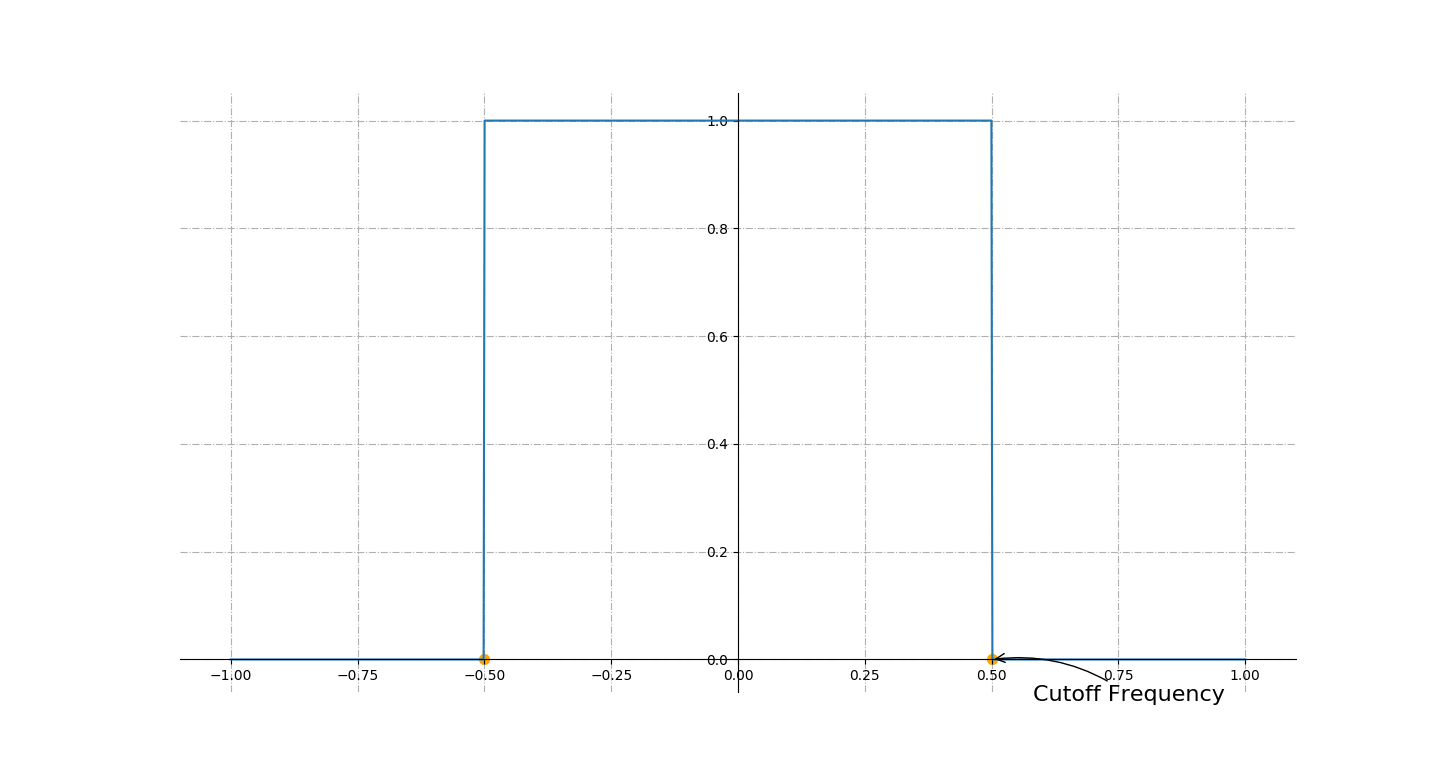
\includegraphics[width=0.4\textwidth]{assets/Figure_5.png}
	\caption{低通滤波器(Low Pass Filter):在时域中的结果相当于与一个特定的$\sinc$函数进行卷积。}
\end{figure}
\begin{figure}[H]
	\centering
	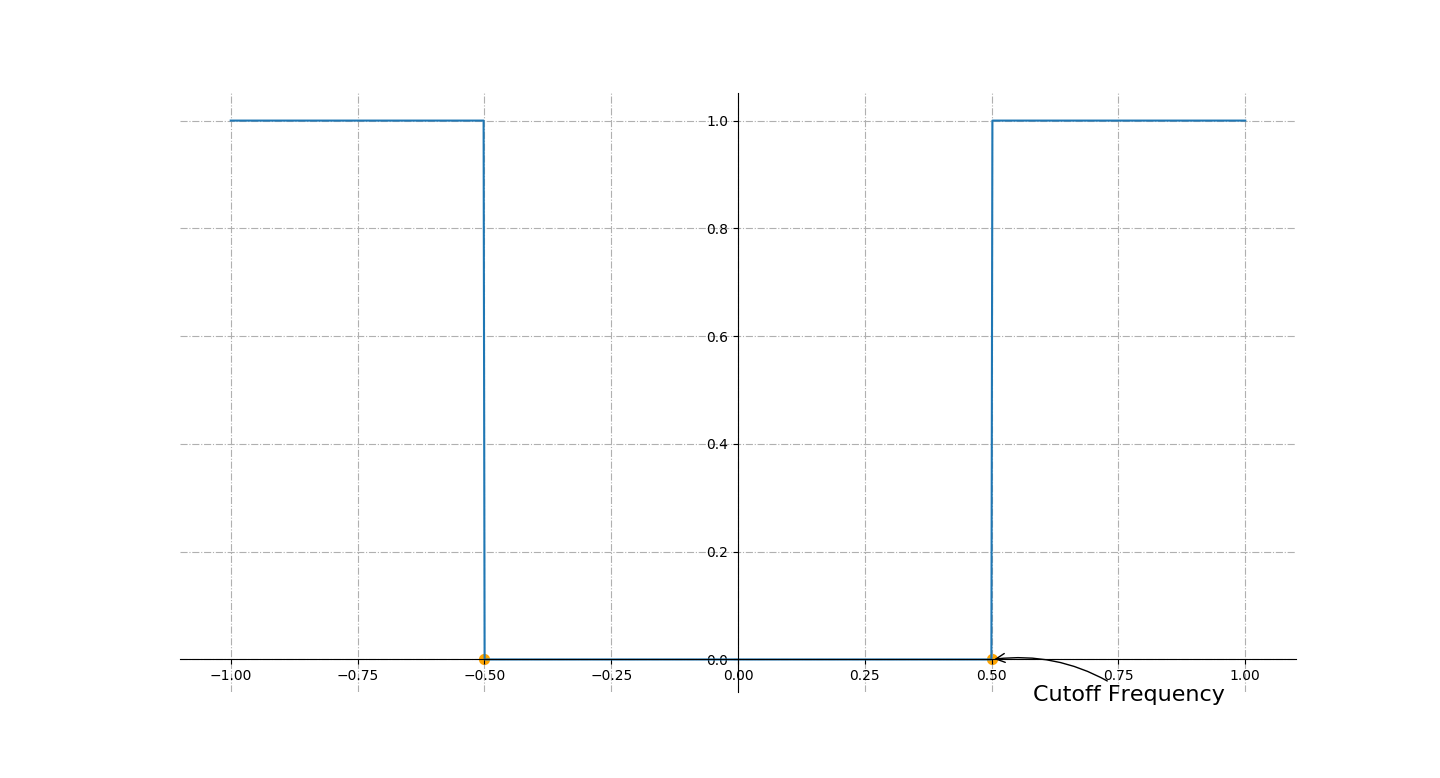
\includegraphics[width=0.4\textwidth]{assets/Figure_6.png}
	\caption{高通滤波器(High Pass Filter)}:常用于边缘检测。
\end{figure}
\begin{figure}[H]
	\centering
	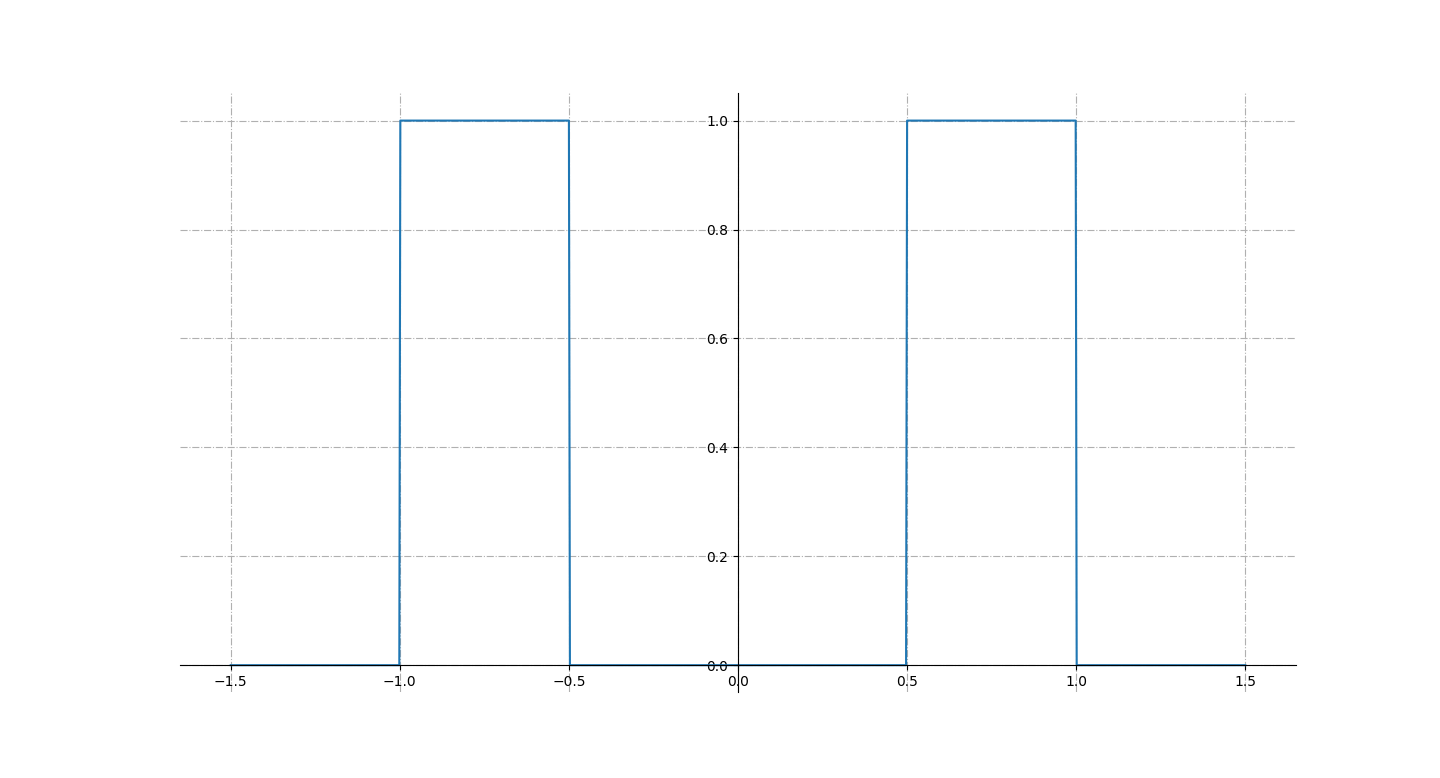
\includegraphics[width=0.4\textwidth]{assets/Figure_7.png}
	\caption{带通滤波器(Band Pass Filter)}
\end{figure}
%TODO:热方程
\section{傅立叶变换的导数定理}
\subsection{$\mathcal{F}f'(s)=2\cdot \pi\cdot i\cdot s\cdot \mathcal{F}f(s)$}
对原函数进行微分后,它的傅立叶变换等于其原函数的傅立叶变换乘以$2\cdot \pi\cdot i\cdot s$。

\begin{align*}
	f(t)                          & =\int_{-\infty}^{\infty}\ \mathcal{F}f(s)\cdot e^{2\cdot \pi\cdot i\cdot s\cdot t}\ ds                                 \\
	\frac{\partial f}{\partial t} & =\int_{-\infty}^{\infty}\ \mathcal{F}f(s)\cdot(2\cdot \pi\cdot i\cdot s\cdot e^{2\cdot \pi\cdot i\cdot s\cdot t})\ ds  \\
	                              & =\int_{-\infty}^{\infty}\ [2\cdot \pi\cdot i\cdot s\cdot \mathcal{F}f(s)]\cdot e^{2\cdot \pi\cdot i\cdot s\cdot t}\ ds
\end{align*}
推广开来有:
$$
	\mathcal{F}f^{(n)}(s)=(2\cdot \pi\cdot i\cdot s)^n\cdot \mathcal{F}f(s)
$$
\subsection{$(f*g)'=f'*g$}
\begin{align*}
	  & \mathcal{F}(f*g)'                                              \\
	= & (2\cdot \pi\cdot i\cdot s)\cdot \mathcal{F}(f*g)               \\
	= & (2\cdot \pi\cdot i\cdot s)\cdot \mathcal{F}f\cdot \mathcal{F}g \\
	= & \mathcal{F}f'\cdot \mathcal{F}g                                \\
	= & f'*g
\end{align*}
\begin{quote}
	Conv. comes into the solution of differential equations because often in solving differential equations if you take the 傅立叶变换, differentiation becomes multiplication. And multiplication in the 频域 becomes conv. in the 时域 on taking Inverse 傅立叶变换.
\end{quote}
$$
	Differentiation\stackrel{FT}\longrightarrow Multiplication\stackrel{IFT}\longrightarrow Conv.
$$
\section{正态分布}
\subsection{正态分布与标准分布}
若随机变量$X$服从一个位置参数为$\mu$,尺度参数为$\sigma$的正态分布,则其概率密度函数为:
$$
	f(x)=\frac{1}{\sigma\sqrt{2\cdot \pi}}\cdot e^{-\frac{(x-\mu)^2}{2\cdot \sigma^2}}
$$

正态分布的数学期望等于其位置参数$\mu$,其标准差等于尺度参数$\sigma$。
\subsection{归一化的高斯函数$f(t)=e^{-\pi\cdot t^2}$}
\subsubsection{对$f(t)=e^{-\pi\cdot t^2}$求$[0,1]$上的积分}
由于高斯函数的变量$t$在幂的位置上,而且是二次方,因此无法用$dt$对其进行积分计算,下面使用极座标法对其进行积分:
\begin{align*}
	  & (\int_{-\infty}^{\infty}\ e^{-\pi\cdot t^2}\ dt)^2                                        \\
	= & \int_{-\infty}^{\infty}\ e^{-\pi\cdot x^2}\ dx\cdot e^{-\pi\cdot y^2}\ dy                 \\
	= & \iint_{-\infty}^{\infty}\ e^{-\pi\cdot (x^2+y^2)}\ dx\ dy                                 \\
	= & \int_0^{2\cdot \pi} \int_0^{\infty}\ e^{-\pi\cdot r^2}\cdot r\ dr\ d\theta                \\
	= & 2\cdot \pi \int_0^{\infty}\ e^{-\pi\cdot r^2}\cdot r\ dr                                  \\
	= & 2\cdot \pi \int_0^{\infty}\ e^{-\pi\cdot r^2}\ d(\frac{1}{2}\cdot r^2)                    \\
	= & \frac{2\cdot \pi}{\pi}\cdot\frac{1}{2}\int_0^{\infty}\ e^{-\pi\cdot r^2}\ d(\pi\cdot r^2) \\
	= & \int_0^{\infty}\ e^{-s}\ ds=1
\end{align*}

\subsubsection{对$f(t)=e^{-\pi\cdot t^2}$求傅立叶变换}
$$
	\mathcal{F}f(s)=\int_{-\infty}^{\infty}\ e^{-2\cdot \pi\cdot i\cdot s\cdot t}\cdot e^{-\pi\cdot t^2}\ dt
$$
这是一个非常难以积分的项,我们需要采用其他巧妙的方法,微分:
\begin{align*}
	  & (\mathcal{F}f)'(s)                                                                                                      \\
	= & \int_{-\infty}^{\infty}\ \frac{d(e^{-2\cdot \pi\cdot i\cdot s\cdot t})}{ds}\cdot e^{-\pi\cdot t^2}\cdot dt              \\
	= & \int_{-\infty}^{\infty}\ -2\cdot\pi\cdot i\cdot t\cdot e^{-2\cdot \pi\cdot i\cdot s\cdot t}\cdot e^{-\pi\cdot t^2}\ dt  \\
	= & i\cdot \int_{-\infty}^{\infty}\ e^{-2\cdot \pi\cdot i\cdot s\cdot t}\cdot(-2\cdot\pi\cdot t\cdot e^{-\pi\cdot t^2})\ dt \\
	= & -2\cdot\pi\cdot s \int_{-\infty}^{\infty}\ e^{-2\cdot \pi\cdot i\cdot s\cdot t}\cdot e^{-2\cdot\pi\cdot t^2}\ dt        \\
	= & -2\cdot\pi\cdot s\cdot \mathcal{F}f(s)
\end{align*}

求解微分方程得:
\begin{align*}
	  & \mathcal{F}f(s)                                                       \\
	= & \mathcal{F}f(0)\cdot e^{-\pi\cdot s^2}                                \\
	= & \int_{-\infty}^{\infty}\ e^{-\pi\cdot t^2}\ dt\cdot e^{-\pi\cdot s^2} \\
	= & e^{-\pi\cdot s^2}
\end{align*}

也就是说归化为$1$的高斯函数的傅立叶变换还是归化为$1$的高斯函数:
\begin{equation}
	\mathcal{F}(e^{-\pi\cdot t^2})=e^{-\pi\cdot s^2}
\end{equation}
\begin{quote}
	傅立叶导数定理:
	\begin{align*}
		\mathcal{F}f'(s)
		=2\cdot\pi\cdot i\cdot s\cdot \mathcal{F}f(s)
	\end{align*}

	注意区分!!!傅立叶导数定理是求$f$导数的傅立叶变换;上面是求$f$的傅立叶变换的导数。
\end{quote}

\section{分布与卷积}
假设有两个独立的随机变量:$x_1$和$x2$,其密度函数分别为$p_1(x_1)$和$p_2(x_2)$。那么$x_1+x_2$的密度函数为$p_{12}(x_{12})$。

设有任意变量$t$,$\Prob(x_1+x_2\leq t)$意为坐标落在阴影部分的概率:
\begin{figure}[H]
	\centering
	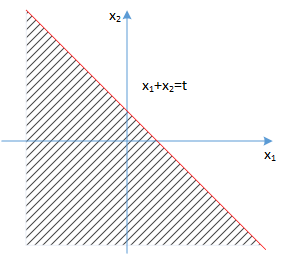
\includegraphics[width=0.4\textwidth]{assets/prob1.png}
	\caption{$x_1,x_2$平面}
\end{figure}
\begin{align*}
	  & \Prob(x_1+x_2\leq t)                                      \\
	= & \iint_{x_1+x_2\leq t}\ p_1(x_1)\cdot p_2(x_2)\ dx_1\ dx_2
\end{align*}

进行变量代换,令$u=x_1$,$v=x_1+x_2$,则:
$$
	\begin{cases}
		x_1 & =u   \\
		x_2 & =v-u \\
		t   & =v
	\end{cases}
$$
进行变量代换后,对应的新平面如下:
\begin{figure}[H]
	\centering
	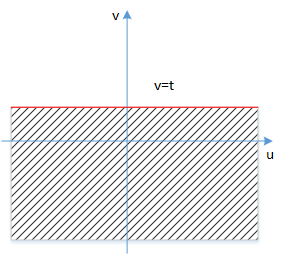
\includegraphics[width=0.4\textwidth]{assets/prob2.png}
	\caption{$u,v$平面}
\end{figure}
\begin{align*}
	  & \Prob(x_1+x_2\leq t)                                                        \\
	= & \Prob(v\leq t)                                                              \\
	= & \int_{-\infty}^{\infty}\ \int_{-\infty}^{t}\ p_1(u)\cdot p_2(v-u)\ du\ dv   \\
	= & \int_{-\infty}^{t}\ (\int_{-\infty}^{\infty}\ p_1(u)\cdot p_2(v-u)\ du)\ dv \\
	= & \int_{-\infty}^{t}\ (p_1*p_2)\ dv
\end{align*}

因此$p_1*p_2$可以作为$x_1+x_2$的密度函数。推广开来就是,独立随机变量的和的密度函数为他们各自密度函数的卷积:
\begin{equation}
	p(x_1+x_2+\cdots+x_n)=p_1*p_2*\cdots *p_n
\end{equation}

\section{傅立叶变换与中心极限定理}
\subsection{中心极限定理}
在适当的条件下,大量相互独立随机变量的均值经适当标准化后依分布收敛于正态分布。
\subsubsection{傅立叶变换中}
%TODO:傅立叶变换中的复指形式的高斯分布和CLT中的高斯分布是什么关系??
在傅立叶变换中我们使用:
$$
	f(t)=e^{-\pi\cdot t^2}
$$
作为标准高斯分布,因为它的傅立叶变换和Inverse 傅立叶变换都是$e^{-\pi\cdot t^2}$。
\subsubsection{CLT中}
标准正态分布的密度函数是:
$$
	p(x)=\frac{1}{\sqrt{2\cdot\pi}}\cdot e^{-\frac{x^2}{2}}
$$

采用这个式子作为标准正态分布的原因是它的均值(期望值)是$0$,它的标准差与方差为$1$。

\subsection{卷积对函数的作用概览}
Several times we've met the idea that 卷积 is a smoothing
operation. Let me begin with somegraphical examples of this,
convolving a discontinuous or rough function repeatedly with itself.
For homework you computed, by hand, the 卷积 of the rectangle
function $\Pi$ with itself a few times.
\begin{figure}[H]
	\centering
	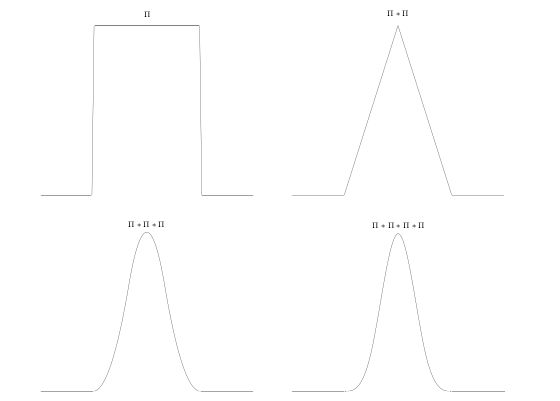
\includegraphics[scale=0.4]{assets/PI.jpg}
	\caption{$\pi$函数做傅立叶变换}
\end{figure}
Not only are the 卷积s becoming smoother, but the
unmistakable shape of a Gaussian is emerging.Is this a coincidence,
based on the particularly simple nature of the function $\Pi$, or
is something more going on? Here is a plot of, literally, a random
function $f(x)$ --- the values $f(x)$ are just randomly chosen
numbers between 0 and 1.

\subsection{中心极限定理的推导过程}
\subsubsection{初始条件}
设有$n$个独立同分布的随机变量:$x_1,x_2,\cdots,x_n$,他们满足以下条件:
\begin{enumerate}
	\def\labelenumi{\arabic{enumi}.}
	\item
	      均值为$0$;
	\item
	      标准差为$1$。
\end{enumerate}
用$s_n$表示这$n$个随机变量的和,则$s_n$的密度函数为:
$$
	p^{*n}=\underbrace{p*p*\cdots *p}_{\text{n个p}}
$$

$S_n$的均值为$0$,标准差为$\sqrt{n}$,因此我们需要对它进行标准化(这里没咋太看懂),标准化后的密度函数为:
$$
	p_{normal}(x)=\sqrt{n}\cdot p^{*n}(\sqrt{n}\cdot x)
$$
\subsubsection{解答}
\begin{align*}
	        & \mathcal{F}p_{normal}(x)                                                                                                                                                     \\
	=       & \mathcal{F}(\sqrt{n}\cdot p^{*n})(\sqrt{n}\cdot x)                                                                                                                           \\
	=       & \sqrt{n}\cdot\frac{1}{\sqrt{n}}\cdot [\mathcal{F}(p^{*n})](\frac{s}{\sqrt{n}})                                                                                               \\
	=       & [\mathcal{F}(p^{*n})](\frac{s}{\sqrt{n}})                                                                                                                                    \\
	=       & (\mathcal{F}p)^n(\frac{s}{\sqrt{n}})                                                                                                                                         \\
	=       & [\int_{-\infty}^{\infty}\ e^{-2\cdot \pi\cdot i\cdot \frac{s}{\sqrt{n}}\cdot x}\cdot p(x)\ dx]^n                                                                             \\
	=       & [\int_{-\infty}^{\infty}\ [1-\frac{2\cdot \pi\cdot i\cdot s\cdot x}{\sqrt{n}}+\frac{1}{2}\cdot (\frac{2\cdot \pi\cdot i\cdot s\cdot x}{\sqrt{n}})^2+\cdots]\cdot p(x)\ dx]^n \\
	=       & [\int_{-\infty}^{\infty}\ p(x)\ dx-\frac{2\cdot \pi\cdot i\cdot s}{\sqrt{n}}\cdot \int_{-\infty}^{\infty}\ x\cdot p(x)\ dx                                                   \\
	-       & \frac{1}{2}\cdot (\frac{2\cdot \pi\cdot i\cdot s}{\sqrt{n}})^2\cdot \int_{-\infty}^{\infty}\ x^2\cdot p(x)\ dx+\cdots]^n                                                     \\
	=       & (1-0-\frac{2\cdot\pi^2\cdot s^2}{n}+\cdots)^n                                                                                                                                \\
	\approx & (1-\frac{2\cdot \pi^2\cdot s^2}{n})^n
\end{align*}

当$n\rightarrow\infty$时:
$$
	\lim\limits_{n\rightarrow\infty}(1-\frac{2\cdot \pi^2\cdot s^2}{n})^n\approx e^{-2\cdot\pi^2\cdot s^2}
$$

即:
$$
	\mathcal{F}(\sqrt{n}\cdot p^{*n})(\sqrt{n}\cdot x)=e^{-2\cdot\pi^2\cdot s^2}
$$
用Inverse 傅立叶变换求出:
\begin{equation}
	p_{normal}=\mathcal{F}^{-1}(e^{-2\cdot\pi^2\cdot s^2})=\frac{1}{\sqrt{2\cdot \pi}}\cdot e^{-\frac{x^2}{2}}
\end{equation}